\documentclass[bachelor, och, coursework]{SCWorks}
% параметр - тип обучения - одно из значений:
%    spec     - специальность
%    bachelor - бакалавриат (по умолчанию)
%    master   - магистратура
% параметр - форма обучения - одно из значений:
%    och   - очное (по умолчанию)
%    zaoch - заочное
% параметр - тип работы - одно из значений:
%    referat    - реферат
%    coursework - курсовая работа (по умолчанию)
%    diploma    - дипломная работа
%    pract      - отчет по практике
% параметр - включение шрифта
%    times    - включение шрифта Times New Roman (если установлен)
%               по умолчанию выключен
\usepackage{subfigure}
\usepackage{tikz,pgfplots}
\pgfplotsset{compat=1.5}
\usepackage{float}

%\usepackage{titlesec}
\setcounter{secnumdepth}{4}
%\titleformat{\paragraph}
%{\normalfont\normalsize}{\theparagraph}{1em}{}
%\titlespacing*{\paragraph}
%{35.5pt}{3.25ex plus 1ex minus .2ex}{1.5ex plus .2ex}

\titleformat{\paragraph}[block]
{\hspace{1.25cm}\normalfont}
{\theparagraph}{1ex}{}
\titlespacing{\paragraph}
{0cm}{2ex plus 1ex minus .2ex}{.4ex plus.2ex}

% --------------------------------------------------------------------------%
\usepackage[T2A]{fontenc}
\usepackage[utf8]{inputenc}
\usepackage{graphicx}
\graphicspath{ {./img/} }
\usepackage{tempora}

\usepackage[sort,compress]{cite}
\usepackage{amsmath}
\usepackage{amssymb}
\usepackage{amsthm}
\usepackage{fancyvrb}
\usepackage{listings}
\usepackage{listingsutf8}
\usepackage{longtable}
\usepackage{array}
\usepackage[english,russian]{babel}

\usepackage[colorlinks=true, linkcolor=black]{hyperref}
\usepackage{url}

\usepackage{underscore}
\usepackage{setspace}
\usepackage{indentfirst} 
\usepackage{mathtools}
\usepackage{amsfonts}
\usepackage{enumitem}
\usepackage{tikz}

\usepackage{minted}
\setminted[python3]{style=bw, linenos, breaklines=true, fontsize=\footnotesize}

\newcommand{\eqdef}{\stackrel {\rm def}{=}}
\newcommand{\specialcell}[2][c]{%
\begin{tabular}[#1]{@{}c@{}}#2\end{tabular}}

\renewcommand\theFancyVerbLine{\small\arabic{FancyVerbLine}}

\newtheorem{lem}{Лемма}

\begin{document}

% Кафедра (в родительном падеже)
\chair{теоретических основ компьютерной безопасности и криптографии}

% Тема работы
\title{Обнаружение сетевого P2P трафика}

% Курс
\course{3}

% Группа
\group{331}

% Факультет (в родительном падеже) (по умолчанию "факультета КНиИТ")
\department{факультета КНиИТ}

% Специальность/направление код - наименование
%\napravlenie{09.03.04 "--- Программная инженерия}
%\napravlenie{010500 "--- Математическое обеспечение и администрирование информационных систем}
%\napravlenie{230100 "--- Информатика и вычислительная техника}
%\napravlenie{231000 "--- Программная инженерия}
\napravlenie{10.05.01 "--- Компьютерная безопасность}

% Для студентки. Для работы студента следующая команда не нужна.
% \studenttitle{Студентки}

% Фамилия, имя, отчество в родительном падеже
\author{Стаина Романа Игоревича}

% Заведующий кафедрой
\chtitle{д. ф.-м. н., доцент} % степень, звание
\chname{М.~Б.~Абросимов}

%Научный руководитель (для реферата преподаватель проверяющий работу)
\satitle{доцент к.ю.н., доцент} %должность, степень, звание
\saname{А.~В.~Гортинский}

% Руководитель практики от организации (только для практики,
% для остальных типов работ не используется)
% \patitle{к.ф.-м.н.}
% \paname{С.~В.~Миронов}

% Семестр (только для практики, для остальных
% типов работ не используется)
%\term{8}

% Наименование практики (только для практики, для остальных
% типов работ не используется)
%\practtype{преддипломная}

% Продолжительность практики (количество недель) (только для практики,
% для остальных типов работ не используется)
%\duration{4}

% Даты начала и окончания практики (только для практики, для остальных
% типов работ не используется)
%\practStart{30.04.2019}
%\practFinish{27.05.2019}

% Год выполнения отчета
\date{2022}

\maketitle

% Включение нумерации рисунков, формул и таблиц по разделам
% (по умолчанию - нумерация сквозная)
% (допускается оба вида нумерации)
% \secNumbering

%-------------------------------------------------------------------------------------------

% \begin{minted}[fontsize=\small]{MySQL}
% \end{minted}

% \begin{figure}[H]
%     \centering
%     \includegraphics[width=0.999\textwidth]{img/}
%     \caption{}
%     \label{easy_hack}
% \end{figure}

\tableofcontents

\intro
С развитием Интернета развивались файлообменные сети, благодаря которым появилась \textbf{P2P} (\textbf{p}eer-\textbf{to}-\textbf{p}eer) "--- одноранговая, децентрализованная или пиринговая сеть. Это распределённая архитектура приложения, которая разделяет задачи между узлами (peer). Узлы имеют одинаковые привилегии в приложении и образуют сеть равносильных узлов.

Узлы делают свои ресурсы, такие как вычислительная мощность, объем диска или пропускная способность, напрямую доступными остальным членам сети, без необходимости координировать действия с помощью серверов. Узлы являются одновременно поставщиками и потребителями ресурсов, в отличие от стандартной клиент-сервер модели, где поставщик и потребитель ресурсов разделены. \cite{P2P_1}

В мае 1999 года, в Интернет с более чем миллионом пользователей, Шон Фэннинг внедрил приложение файлообменник Napster. 
Napster стал началом P2P-сети, такой какую мы знаем её сейчас, пользователи участвуют в создании виртуальной сети, 
полностью независимой от физической, без администрирования и каких-либо ограничений.

Концепция вдохновила новую философию во многих областях человеческого взаимодействия. 
P2P-технология позволяет пользователям интернета образовывать группы и коллаборации, формируя, тем самым, пользовательские поисковые движки, виртуальные суперкомпьютеры и файловые системы. 
Видение Всемирной паутины Тима Бернерса-Ли было близко к P2P-сети, в том смысле, 
что каждый пользователь является активным создателем и редактором контента.

В тоже время с появлением P2P появилась необходимость обнаруживать соотвествующий трафик в сети.
Универсального способа обнаружения работающего P2P-приложения нет. С развитием файлообменных сетей стало затруднительно
идентифицировать P2P-трафик с помощью номеров портов. Появилась необходимость исследования трафика на основании поведения узлов сети. Однако даже поведение такого трафика, его сигнатура и прочие признаки также могут изменяться со временем, поэтому все существующие методы должны обновляться и усовершенствоваться, чтобы поспевать за развитием P2P-приложений.


\section{Архитектура} 
P2P-сеть строится вокруг понятия равноправных узлов "--- клиенты и серверы одинаково взаимодействуют с другими узлами сети. 
Такая модель построения сети отличается от модели клиент-сервер, где взаимодействие идет с центральным сервером. 
На рисунке \ref{image1} а) изображены архитектура клиент-сервера и б) архитектура P2P. 
Типичным примером передачи файла в модели клиент-сервер является File Transfer Protocol (FTP), 
в котором программы клиента и сервера разделены: клиент инициирует передачу, а сервер отвечает на запросы. 

\begin{figure}[h]
    \begin{minipage}[h]{0.49\linewidth}
        \center{\includegraphics[width=0.75\linewidth]{arch_client-server.png} \\ а)}
    \end{minipage}
    \hfill
    \begin{minipage}[h]{0.49\linewidth}
        \center{\includegraphics[width=0.75\linewidth]{arch_p2p.png} \\ б)}
    \end{minipage}
    \caption{Архитектура клиент-сервера и P2P}
    \label{image1}
\end{figure}

\subsection{Базовые элементы P2P-сетей}
\subsubsection{Узел P2P-сети}
\textbf{Узел (Peer)} "--- фундаментальный составляющий блок любой одноранговой сети. 
Каждый узел имеет уникальный идентификатор и принадлежит одной или нескольким группам. 
Он может взаимодействовать с другими узлами как в своей, так и в других группах. \cite{P2P_2}

Виды узлов:
\begin{itemize}
    \item \textbf{Простой узел}. Обеспечивает работу конечного пользователя, предоставляя ему сервисы других узлов и	
    обеспечивая предоставление ресурсов пользовательского компьютера другим	участникам сети.
    \item \textbf{Роутер}. Обеспечивает механизм взаимодействия между узлами, отделёнными от сети брандмауэрами или NAT-системами.	
\end{itemize}

\subsubsection{Группа узлов}
\textbf{Группа узлов} "--- набор узлов, сформированный для решения общей задачи или достижения общей цели. 
Могут предоставлять членам своей группы такие наборы сервисов, которые недоступны узлам, входящим в другие группы.

Группы узлов могут разделяться по следующим признакам:
\begin{itemize}
    \item приложение, ради которого они объединены в группу;
    \item требования безопасности;
    \item необходимость информации о статусе членов группы.
\end{itemize}

\subsubsection{Сетевой транспорт}
\textbf{Конечные точки (Endpoints)} "--- источники и приёмники любого массива данных передаваемых по сети.

\textbf{Пайпы (Pipes)} "--- однонаправленные, асинхронные виртуальные коммуникационные каналы, соединяющие две или более конечные точки.

\textbf{Сообщения} "--- контейнеры информации, которая передаётся через пайп от одной конечной точки до другой.

\subsection{Маршрутизация}
P2P относят к прикладному уровню сетевых протоколов, а P2P-сети обычно реализуют некоторую форму виртуальной (логической) сети, наложенной поверх физической, то есть описывающей реальное расположение
и связи между узлами, такой сети, где узлы образуют подмножество узлов в физической сети. 
Данные по-прежнему обмениваются непосредственно над базовой TCP/IP сетью, 
а на прикладном уровне узлы имеют возможность взаимодействовать друг с другом напрямую, 
с помощью логических связей. Наложение используется для индексации и обнаружения узлов, 
что позволяет системе P2P быть независимой от физической сети. На основании того, как узлы соединены 
друг с другом внутри сети, и как ресурсы индексированы и расположены, сети классифицируются на 
\textbf{неструктурированные} и \textbf{структурированные} (или как их \textbf{гибрид}).

\subsubsection{Неструктурированные сети}
Неструктурированная Р2Р сеть не формирует определенную структуру сети, а случайным образом соединяет узлы друг с другом. 
Неструктурированные сети легко организуются и доступны для локальных оптимизаций, так как не существует глобальной структуры формирования сети.
Кроме того, поскольку роль всех узлов в сети одинакова, неструктурированные сети являются весьма надежными в условиях, 
когда большое количество узлов часто подключаются к сети или отключаются от неё.

Однако из-за отсутствия структуры возникают некоторые ограничения. 
В частности, когда узел хочет найти нужный фрагмент данных в сети, поисковый запрос должен быть направлен через сеть, 
чтобы найти как можно больше узлов, которые обмениваются данными. Такой запрос вызывает очень высокое количество сигнального трафика в сети, 
требует высокой производительности и не гарантирует, что поисковые запросы всегда будут решены.

\subsubsection{Структурированные сети}
В структурированных Р2Р-сетях наложение организуется в определенную топологию, и протокол гарантирует, 
что любой узел может эффективно участвовать в поиске файла или ресурса, даже если ресурс использовался крайне редко.

Наиболее распространенный тип структурированных сетей P2P реализуется распределенными хэш-таблицами (DHT), 
в котором последовательное хеширование используется для привязки каждого файла к конкретному узлу. Это позволяет узлам искать ресурсы в сети, используя хэш-таблицы, хранящие пару ключ-значение, и любой участвующий узел может эффективно извлекать значение, связанное с заданным ключом.

Тем не менее, для эффективной маршрутизации трафика через сеть, узлы структурированной сети должны обладать списком соседей, которые удовлетворяют определенным критериям. 
Это делает их менее надежными в сетях с высоким уровнем оттока абонентов (т.е. с большим количеством узлов, 
часто подключающихся к сети или отключающихся от нее).

\subsubsection{Гибридные модели}
Гибридные модели представляют собой сочетание Р2Р-сети и модели клиент-сервер. 
Гибридная модель должна иметь центральный сервер, который помогает узлам находить друг друга. 
Есть целый ряд гибридных моделей, которые находят компромисс между функциональностью, обеспечиваемой структурированной сетью модели клиент-сервер, 
и равенством узлов, обеспечиваемым чистыми одноранговыми неструктурированными сетями. 
В настоящее время гибридные модели имеют более высокую производительность, чем чисто неструктурированные или чисто структурированные сети.

\subsection{Безопасность}
Как и любая другая форма программного обеспечения, P2P-приложения могут содержать уязвимости. 
Особенно опасным для P2P программного обеспечения, является то, что Р2Р-приложения действуют и в качестве серверов, и в качестве клиентов, а это означает, что они могут быть более уязвимы для удаленных эксплоитов.

\subsubsection{Маршрутизационные атаки}
Поскольку каждый узел играет роль в маршрутизации трафика через сеть, злоумышленники могут выполнять различные <<маршрутизационные атаки>> или атаки отказа в обслуживании. Примеры распространенных атак маршрутизации включают в себя <<неправильную маршрутизацию поиска>>, когда вредоносные узлы преднамеренно пересылают запросы неправильно или возвращают ложные результаты, <<неправильную маршрутизацию обновления>>, когда вредоносные узлы изменяют таблицы маршрутизации соседних узлов, посылая им ложную информацию, и <<неправильную маршрутизацию разделения сети>>, когда новые узлы подключаются через вредоносный узел, который помещает новичков в разделе сети, заполненной другими вредоносными узлами.

\subsubsection{Поврежденные данные и вредоносные программы}
Распространенность вредоносных программ варьируется между различными протоколами одноранговых сетей. 
Исследования, анализирующие распространение вредоносных программ по сети P2P, обнаружили, например, что 63\% запросов на загрузку по сети Limewire содержали некоторую форму вредоносных программ, в то время как на OpenFT только 3\% запросов содержали вредоносное программное обеспечение. Другое исследование анализа трафика в сети Kazaa показало, что 15\% от 500 000 отобранных файлов были инфицированы одним или несколькими из 365 различных компьютерных вирусов.

Поврежденные данные также могут быть распределены по P2P-сети путем изменения файлов, которые уже были в сети. 
Например, в сети FastTrack, RIAA удалось внедрить фальшивые данные в текущий список загрузок и в уже загруженные файлы (в основном файлы MP3). 
Файлы, инфицированные вирусом RIAA, были непригодны впоследствии и содержали вредоносный код. 
Следовательно, P2P-сети сегодня внедрили огромное количество механизмов безопасности и проверки файлов. 
Современное хеширование, проверка данных и различные методы шифрования сделали большинство сетей устойчивыми к 
практически любому типу атак, даже когда основные части соответствующей сети были заменены фальшивыми или нефункциональными узлами.

\subsection{Отказоустойчивость и масштабируемость сети}
Децентрализованность Р2Р-сетей повышает их надежность, так как этот метод взаимодействия устраняет ошибку единой точки разрыва, присущую клиент-серверным моделям. С ростом числа узлов объем трафика внутри системы увеличивается, масштаб сети так же увеличивается, что приводит к уменьшению вероятности отказа. Если один узел перестанет функционировать должным образом, то система в целом все равно продолжит работу. 
В модели клиент-сервер с ростом количества пользователей уменьшается количество ресурсов выделяемых на одного пользователя, что приводит к риску возникновения ошибок.

\subsection{Распределенное хранение и поиск}
Возможность резервного копирования данных, восстановление и доступность приводят как к преимуществам, так и к недостаткам Р2Р-сетей. 
В централизованной сети только системный администратор контролирует доступность файлов. 
Если администраторы решили больше не распространять файл, его достаточно удалить с серверов,
и файл перестанет быть доступным для пользователей. Другими словами, клиент-серверные модели имеют возможность управлять доступностью файлов. В Р2Р-сети доступность контента определяется степенью его популярности, так как поиск идет по всем узлам, через которые файл проходил. 
То есть, в Р2Р-сетях нет централизованного управления как системного администратора в клиент-серверном варианте, 
а сами пользователи определяют уровень доступности файла.

\section{Применение P2P}
В Р2Р сетях, пользователи передают и используют контент сети. Это означает, что, в отличие от клиент-серверных сетей, 
скорость доступа к данным возрастает с увеличением числа пользователей, использующих этот контент. 
На этой идее построен протокол Bittorrent "--- пользователи, скачавшие файл, становятся узлами и помогают другим пользователям скачать файл быстрее. 
Эта особенность является главным преимуществом Р2Р сетей.

Множество файлообменных систем, таких как Gnutella, G2 и eDonkey популяризовали Р2Р технологии:
\begin{itemize}
    \item Пиринговые системы распространения контента.
    \item Пиринговые системы обслуживания, например, повышение производительности, в частности, Correli Caches.
    \item Публикация и распространение программного обеспечения (Linux, видеоигры).
\end{itemize}

В связи децентрализованностью доступа к данным в Р2Р сетях возникает проблема нарушения авторских прав. 
Компании, занимающиеся разработкой Р2Р приложений часто принимают участие в судебных конфликтах. 
Самые известные судебные дела это Grokster против RIAA и MGM Studios, Inc. против Grokster Ltd., 
где в обоих случаях технологии файлообменных систем признавались законными.

\section{Обнаружение P2P трафика без анализа полезной нагрузки}
\subsection{Анализ портов}
Многие P2P-приложения работают на определённых портах. 
Некоторые из таких указаны в таблице \ref{table:p2p-ports} \cite{p2p-list}.

\begin{table}[H]
    \caption{Список наиболее известных портов, используемых P2P-протоколами}
    \label{table:p2p-ports}
    \begin{center}
    {\small
    \begin{tabular}{|c|c|c|c|c|c|c|c|c|}
        \hline
    Протоколов   & Номера TCP/UDP портов \\ \hline
    Bittorrent      & 6881-6999  \\ \hline
    Direct Connect  & 411, 412, 1025-32000  \\ \hline
    eDonkey         & 2323, 3306, 4242, 4500, 4501, 4661-4674, 4677, 4678, 4711, 4712, 7778  \\ \hline
    FastTrack       & 1214, 1215, 1331, 1337, 1683, 4329  \\ \hline
    Yahoo           & 5000-50010, 5050, 5100  \\ \hline
    Napster         & 5555, 6257, 6666, 6677, 6688, 6699-6701  \\ \hline
    MSN             & 1863, 6891-6901 \\ \hline
    MP2P            & 10240-20480, 22321, 41170  \\ \hline
    Kazaa           & 1214  \\ \hline
    Gnutella        & 6346, 6347  \\ \hline
    ARES Galaxy     & 32285  \\ \hline
    AIM             & 1024-5000, 5190  \\ \hline
    \end{tabular}
    }
    \end{center}
\end{table}

Для реализации данного метода достаточно обнаружить в сетевом трафике соединения, использующие такие порты.
Очевидно, что данный способ легко реализовать, однако он имеет недостатки. Во-первых, многие приложения могут
использовать случайные порты, или же пользователь может сам выбрать номер порта. Во-вторых, такие порты могут использоваться не P2P-приложениями и наоборот, P2P-приложения могут использовать номера портов известных приложений, например, 80 или 443 порты "--- HTTP и HTTPS. Так, в работе \cite{30percent}
приведены результаты, которые показывают, что зачастую на основе данного метода можно определить лишь 30\% P2P трафика.

\subsection{Анализ сигнатур}
Суть этого способа заключается в мониторинге трафика, проходящего через сеть, 
на предмет обнаружения определенных \textbf{сигнатур}, специфичных для P2P-приложений, в полезной нагрузке пакетов \cite{seclab}.
Сетевая сигнатура "--- набор данных, которые необходимо найти в трафике. Это могут быть IP-адреса, порты, флаги (например, протокола TCP) и так далее. Многие современные коммерческие и свободно распространяемые решения для обнаружения P2P-трафика основаны на этом методе. Например, система предотвращения вторжений Snort предоставляет возможность создавать набор правил, включающих информацию о характеристиках транспортного уровня и содержимом полезной нагрузки пакетов для различных приложений. 

Особенности данного метода:
\begin{itemize}
    \item Необходимо постоянное обновление базы сигнатур.
    \item Трафик зачастую зашифрован, что сильно затрудняет анализ.
    \item Поиск сигнатур на прикладном сетевом уровне очень ресурсоёмкий.
\end{itemize}

\subsection{Эвристические предположения}

\subsubsection{TCP/UDP-эвристика}
Если в течение интервала времени обнаружено, что пара адресов взаимодействует и по TCP-, и по UDP-протоколу, то они
предположительно участвуют в P2P-обмене.

\subsubsection{IP/Port-эвристика}
Ещё одной особенностью P2P является тот факт, что при обращении к паре (IP-назначения, порт-назначения)
количество адресов источников практически совпадает с количеством портов источников. Подобное поведение
характерно, например, для сигнального взаимодействия с раздающим данные Bittorrent-клиентом. Однако стоит отметить,
что такое поведение характерно не только для P2P.

\section{Идентификация Bittorrent}
В работе \cite{bittorrent} предложен алгоритм, который основывается на четырёх критериях.

\subsection{Подключенные IP-адреса}
Первый критерий основан на IP/Port-эвристике. Хосты Bittorrent всегда подключены ко многим IP-адресам.
Под подключенными IP-адресами понимается, что они передали друг другу хотя бы
по одному TCP-пакету. В Bittorrent это может быть необходимо для подключения к раздаче и передачи особенных
сообщений (choke, have, keepalive). Причём каждый пир (участник) пытается поддерживать не менее 20 пиров, следовательно,
каждый пир периодически отправляет несколько TCP-пакетов на один и тот же набор IP-адресов.

\subsection{Передача данных}
Bittorrent разбивает исходные файлы на небольшие части, поэтому пользователи могут скачивать разные файлы
от разных пользователей. Это можно определить по значимому соотношению активных передач. Под активной передачей
подразумевается хотя бы 5 больших TCP-пакетов, т.е. размер пакета должен быть примерно равен \textit{MTU} (максимальная единица передачи). В Ethernet это около 1500 байт. Передача пакетов максимального размера необходима для того, 
чтобы их количество было минимальным для передачи файла.

Однако пиры Bittorrent не всегда одновременно обмениваются данными между собой. 
Это связано с \textit{алгоритмом дросселирования} (\textit{choke}). Этот алгоритм выбирает соседей, которым будут раздаваться или с которых будут скачиваться файлы. В любой момент времени пир загружает данные не более, чем 
с 4 пиров, которые обеспечивают самую высокую скорость загрузки. % там ещё предложение есть
 
\subsection{Двусторонняя передача данных}
Процесс выбора в алгоритме дросселирования приводит к двусторонней передаче данных. В отличие от Bittorrent, другие 
интернет-приложения обычно работают по схеме клиент-сервер, поэтому данные передаются только в одном направлении в 
определённый промежуток времени. Кроме того, в других протоколах P2P-обмена между элементами нет взаимного обмена,
который заложен в алгоритме дросселирования. Пирам в этих протоколах не нужно загружать свои фрагменты другим пирам,
с которых они скачивают данные. 

\subsection{Изменение отношений}
В алгоритме дросселирования все пиры в наборе сортируются каждые 10 секунд в порядке убывания скорости загрузки данных.
После сортировки локальный пир будет раздавать данные только первым четырём пирам в отсортированном списке.
Учитывая, что скорость передачи довольно динамична, выбранные пиры будут часто меняться. Таким образом, пара пиров
может активно передавать данные друг другу, но потом внезапно может стать неактивной. В результате хост Bittorrent может
быть идентифицирован по значимому соотношению изменений IP-отношений к активным передачам.

\subsection{Алгоритм}
На основании четырёх критериев создаются специальные метрики, которые рассчитываются каждые 30 секунд
и сравниваются с пороговым значением, чтобы определить, является ли хост пиром Bittorrent. В данном алгоритме
обрабатываются только TCP-пакеты. 

\subsubsection{Подключения}
Подсчитывается число $C$ "--- количество пиров, которые общались с хостом. Если это количество будет больше или равно порогу $C_{threshold}$, то хост будет идентифицирован как Bittorrent-хост.
\[ C \geq C_{threshold} \]

\subsubsection{Коэффициент активной передачи}
Коэффициент активной передачи хоста $R_{AT}$ "--- отношение числа активных подключений $AT$ к общему числу подключений $C$.
Если этот коэффициент больше или равен пороговому $R_{ATthreshold}$, то хост будет идентифицирован как Bittorrent-хост.
\[ R_{AT} \geq R_{ATthreshold}, \]
где $R_{AT} = \frac{AT}{C}$.

\subsubsection{Двусторонние передачи данных}
Измеряется количество подключений $BiAT$, по которым одновременно принимаются и отправляются данные. 
Если это число больше или равно пороговому $BiAT_{threshold}$, то хост будет идентифицирован как Bittorrent-хост.
\[ BiAT \geq BiAT_{threshold} \]

\subsubsection{Коэффициент изменений отношений}
Коэффициент изменений отношений $R_{RC}$ "--- отношение числа изменений отношений $RC$ к числу активных передач $AT$.
Если этот коэффициент больше или равен пороговому $R_{RCthreshold}$, то хост будет идентифицирован как Bittorrent-хост.
\[ R_{RC} \geq R_{RCthreshold}, \]
где $R_{RC} = \frac{RC}{AT}$.

\subsubsection{Точность алгоритма}
Точность данного алгоритма зависит от выбранных пороговых значений. Они могут быть получены эмпирическим путём.
% надо добавить

\section{Описание программы}
В данной работе был разработан \textbf{сниффер} "--- анализатор сетевого трафика. 
Программа выводит на экран информацию о перехваченных пакетах таких сетевых протоколов как \textit{IPv4}, \textit{TCP} и \textit{UDP}. 
Дополнительно последний вывод программы сохраняется в текстовые файлы. Программа обрабатывает трафик, проходящий через сетевой интерфейс, указанный как аргумент при её запуске. По умолчанию в программе указан интерфейс \textit{enp0s3}.

\begin{minted}{python3}
    sudo ./window.py enp0s3
\end{minted}

Для указанного сетевого интерфейса программа включает неразборчивый режим.

При запуске \texttt{window.py} создаётся \textbf{сокет} "--- программный интерфейс для обеспечения обмена данными между процессами. Через него проходит весь сетевой трафик на той виртуальной машине, на которой он находится. 

\begin{minted}[fontsize=\footnotesize]{python3}
    ret = os.system("ip link set {} promisc on".format(interface))

    conn = socket.socket(socket.AF_PACKET, socket.SOCK_RAW, socket.ntohs(3))
    conn.bind((interface, 0))
\end{minted}

\subsection{Функция call_sniff}
Функция \texttt{call_sniff} вызывает функцию \texttt{sniff} из \texttt{sniffer.py}, которая передаёт информацию о пакете для вывода на экран. Эта информация сохраняется в список \texttt{out}. Затем информация о пакетах выводится на экран и сохраняется в текстовый файл \texttt{out.txt}, а списки обнаруженных адресов, взаимодействующих через P2P, сохраняются в \texttt{ip_list.txt}.

\begin{minted}[fontsize=\footnotesize]{python3}
    def call_sniff(self):
        out = sniffer.sniff(conn)
        if out:
            # Вывод времени
            time = str(datetime.now().strftime('%H:%M:%S')) + ":\n"
            if time != self.last_time:
                self.output.insert('end', time)
                file.write(time)
            self.last_time = time

            # Вывод информации о пакете
            for s in out:
                file.write(s)
                self.output.insert('end', s)
            file.write('\n')
            self.output.insert('end', '\n')

        root.after(100, self.call_sniff)  # сканирование каждые 0.1 сек
\end{minted}

Функция \texttt{call_sniff} вызывается каждые 0.1 секунды, то есть сканирование происходит раз в 0.1 секунды.
Эмпирически было установлено, что для анализирования трафика пары приложений, одно из которых взаимодействует через P2P достаточно сканировать раз в 0.2-0.3 секунды. Однако при более активном трафике сканирование следует проводить чаще, чтобы не было пакетов, которые не оказались бы перехваченными.

\subsection{Функция sniff}
Функция \texttt{sniff} обрабатывает информацию о пакете и сохраняет некоторые данные с помощью функции \texttt{save} в глобальные переменные.
В множества \texttt{TCP_addrs} и \texttt{UDP_addrs} сохраняются пары IP-адресов вида (IP-отправителя, IP-получателя), взаимодействующих по соответствующим протоколам.
В множество \texttt{rejected} добавляются IP-адреса с портами, если порт является одним из перечисленных в списке портов-исключений \texttt{EXCEPTIONS}. 
Это необходимо, чтобы отсечь их при дальнейшем анализе, поскольку их активность схожа с P2P-активностью или порт является известным. Например, это могут быть почтовые, игровые или \textit{DNS} сервисы. 

В словарь \texttt{dict_ipport} сохраняются пары вида (\texttt{dest_ip} + \texttt{dest_port} $\to$ объект класса \texttt{IPPort}). 
В таких объектах сохраняется информация о различных адресах источника и различных портах источника для каждой пары адреса назначения (\texttt{dest_ip} + \texttt{dest_port}).

\begin{minted}[fontsize=\footnotesize]{python3}
def sniff(conn):
    output = ''
    raw_data, addr = conn.recvfrom(65536)
    dest_mac, src_mac, eth_proto, data = ethernet_frame(raw_data)

    # IPv4
    if eth_proto == 8:
        (version, header_length, ttl, proto, src, dest, data) = ipv4_packet(data)

        # TCP
        if proto == 6:
            src_port, dest_port, sequence, ack, flag_urg, flag_ack, \
            flag_psh, flag_rst, flag_syn, flag_fin, data = tcp_segment(data)

            output = [TAB_1, 'TCP: ', src, ':', str(src_port), ' -> ', dest,  ':',
                      str(dest_port),  ', ',  str(len(data)), ' Б']

            save(True, src, dest, src_port, dest_port)
            check_ports(src, dest, src_port, dest_port)

        # UDP
        elif proto == 17:
            src_port, dest_port, length, data = udp_segment(data)

            output = [TAB_1, 'UDP: ', src,  ':', str(src_port), ' -> ', dest,  ':',
                      str(dest_port),  ', ',  str(len(data)), ' Б']

            check_ports(src, dest, src_port, dest_port)
            save(False, src, dest, src_port, dest_port)

    return output
\end{minted}

\subsection{Определение P2P трафика}
\subsubsection{Метод анализирования портов}
С помощью функции \texttt{check_ports}, которая вызывается при каждом запуске \texttt{sniff}, проводится анализ портов. 
Если был обнаружен порт, который присутствует в списке \texttt{LIST_P2P}, то IP-адрес вместе с портом заносится в \texttt{p2p_pairs_p}.

\begin{minted}[fontsize=\footnotesize]{python3}
def check_ports(src, dest, src_port, dest_port):
    if LIST_P2P.get(src_port, False):
        p2p_pairs_p.add((src, src_port))
    elif LIST_P2P.get(dest_port, False):
        p2p_pairs_p.add((dest, dest_port))
\end{minted}

В списке пар порт-приложение \texttt{LIST_P2P} находится информация об используемых портах некоторых P2P-приложений, а именно:

\begin{itemize}
    \item Bittorrent;
    \item Direct Connect;
    \item eDonkey;
    \item FastTrack;
    \item Yahoo;
    \item Napster;
    \item Gnutella;
    \item AIM;
    \item Skype;
    \item Steam;
    \item Hamachi;
    \item Radmin VPN;
\end{itemize}

\subsubsection{Метод анализирования потоков}
Данный метод реализуется в функции \texttt{find_p2p}:

\begin{minted}[fontsize=\footnotesize]{python3}
def find_p2p():
    # 1 Заполнение p2p_addrs адресами, взаимодействующими одновременно по TCP и UDP с учётом исключений
    inter = TCP_addrs & UDP_addrs
    for pair_addrs in inter:
        for ipport in rejected:
            if pair_addrs[0] != ipport[0] and pair_addrs[1] != ipport[0]:
                p2p_addrs.add(pair_addrs)

    # 2 Заполнение p2p_addrs адресами, выбранными исходя из check_p2p с учётом исключений
    for ipport in dict_ipport:
        ipp = dict_ipport[ipport]
        ipp.add_to_p2p_addrs1()  # Заполнение массива p2p_addrs1
        ip = ipp.dst_ip
        port = ipp.dst_port
        if ipp.check_p2p() and (ip, port) not in rejected:
            p2p_pairs_ipp.add((ip, port))
\end{minted}

Данная функция работает по следующему алгоритму \cite{algorithm}:

\underline{Шаг 1} (проверка TCP/UDP-эвристики). 
Рассматриваются пары адресов, взаимодействующих одновременно по протоколам \textit{TCP} и \textit{UDP}. 
Если при этом IP-адреса не входят в список исключений \textit{rejected}, то эта пара адресов заносится в массив \texttt{p2p_addrs}.

\underline{Шаг 2} (проверка IP/Port-эвристики). 
Для каждой пары адресов из \texttt{dict_ipport} проверяется, что IP-адрес с портом не находится в списке исключений, и проверяется условие "--- если массив различных адресов источника \texttt{IPSet} содержит более двух адресов, а разница между количеством элементов этого массива и массива различных портов \texttt{PortSet}
источника меньше двух (или меньше 10, если порт является исключением, т.е. находится в списке \texttt{EXCEPTIONS}), то считается, что пара принимает участие в P2P-деятельности и добавляется в \texttt{p2p_pairs_ipp}.

Эти действия проводятся каждые 15 секунд с момента запуска программы.

\subsection{Тестирование программы}
Тестирование программы проводилось по следующей схеме: на хостовой машине с \textit{Windows 10} была запущена виртуальная машина с помощью \textit{Virtual Box}. На виртуальной машине установлена \textit{Manjaro Linux}. Между виртуальной и хостовой машиной сетевой мост с неразборчивым режимом. Программа запущена на виртуальной машине, а проверяемые P2P-приложения на хостовой (рисунок \ref{test1}).

\begin{figure}[H]
    \centering
    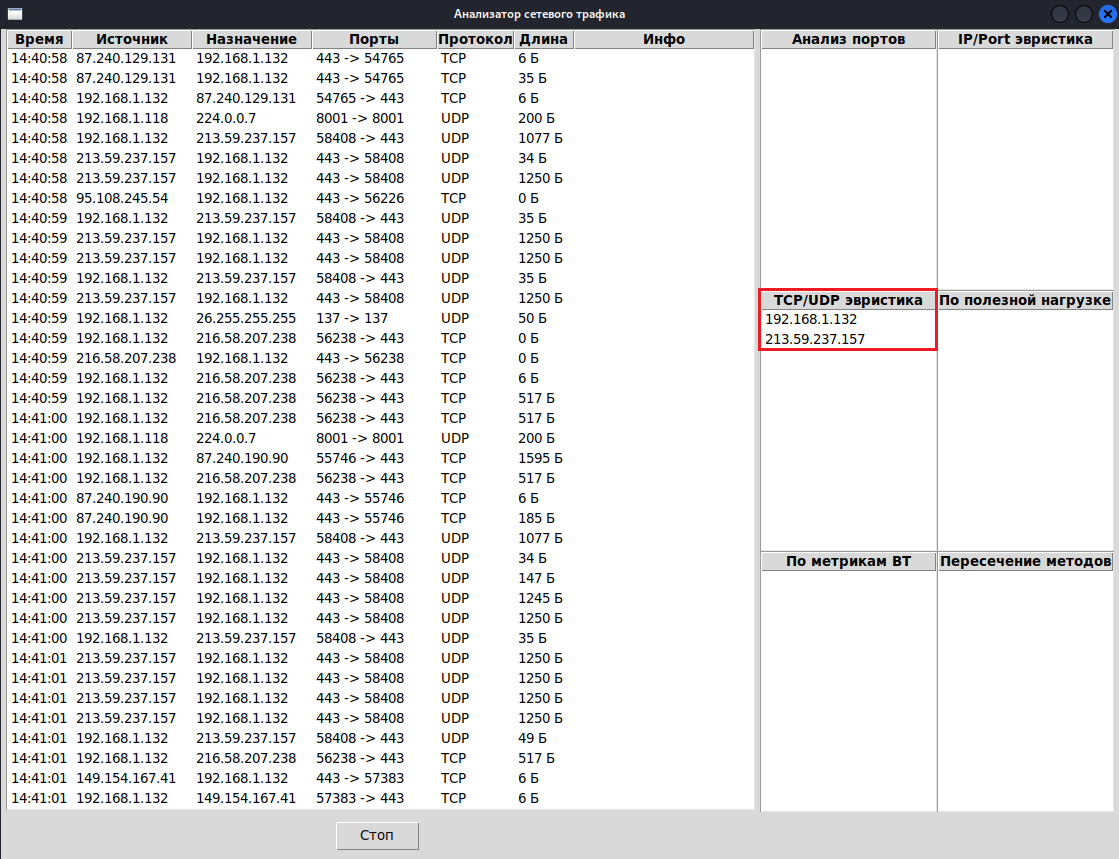
\includegraphics[width=0.999\textwidth]{test1.png}
    \caption{Демонстрация схемы тестирования}
    \label{test1}
\end{figure}

\subsubsection{Запуск программы при отсутствии P2P-активности}
Ни на одной из машин не запущено ни одно P2P-приложение. На виртуальной машине запущено видео на \textit{Youtube}.

На рисунке \ref{test2} видно, что присутствуют ложные срабатывания обнаружения P2P-активности. Анализ портов и TCP/UDP-эвристика дали ложный положительный результат.

Адрес 239.255.255.250:1900 обнаружен ложно, поскольку порт 1900 применяется протоколами SSDP и UPnP для обнаружения новых устройств в локальной сети. В качестве одного из методов обнаружения поддерживается M-SEARCH, подразумевающий отправку multicast-запросов по адресу \\ 239.255.255.250. \cite{IANA}

\begin{figure}[H]
    \centering
    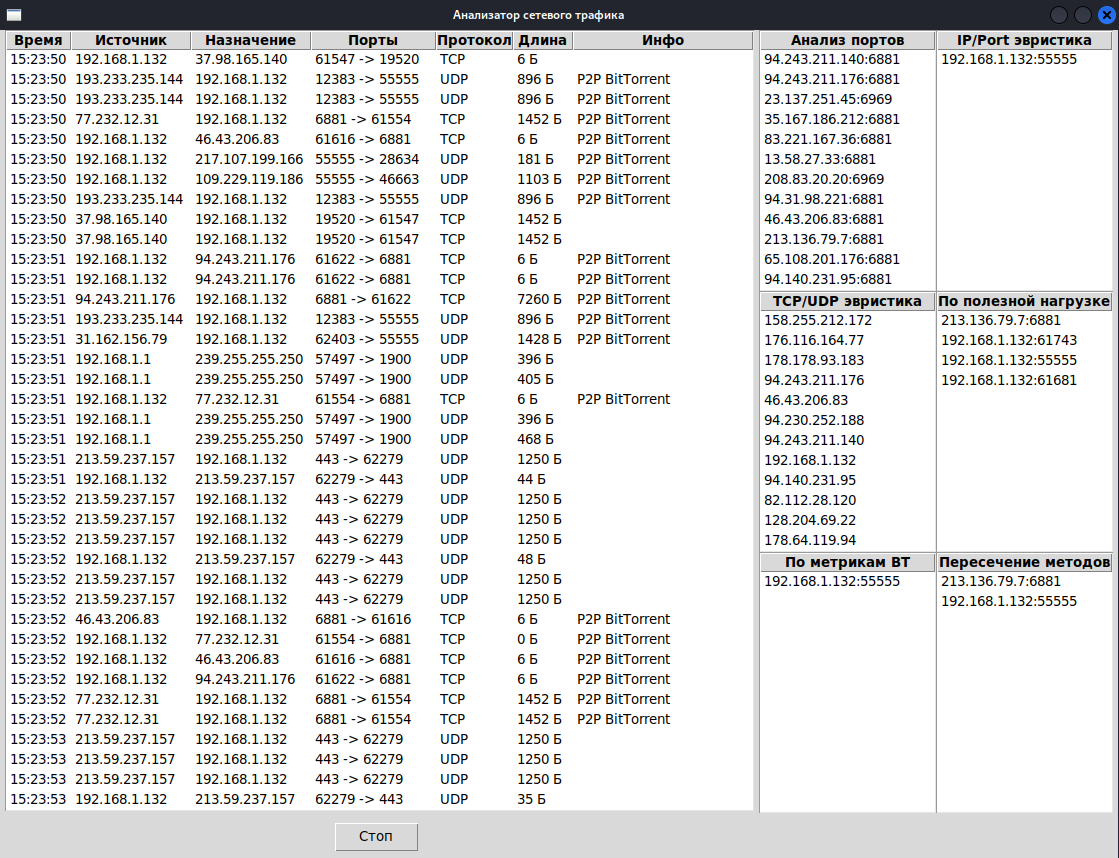
\includegraphics[width=0.999\textwidth]{test2.png}
    \caption{Тестирование программы при запущенном видео на \textit{Youtube}}
    \label{test2}
\end{figure}

\subsubsection{Запуск программы при запущенном клиенте Bittorrent}
На хостовой машине запущен \textit{qBittorrent}. 

На рисунке \ref{test3} видно, что методом анализирования портов была обнаружена P2P-активность. Порты 6881-6889 относятся к Bittorrent. С помощью IP/Port-эвристики был обнаружен адрес 192.168.1.142:27309. IP данного адреса принадлежит хостовой машине, а порт является портом для входящих соединений в клиенте qBittorrent (рисунок \ref{btport}). Данный порт является случайным, поэтому методом анализирования портов его не удалось бы обнаружить. Также TCP/UDP-эвристика показывает достаточно большое количество пар адресов, между которым была обнаружена P2P-активность.

\begin{figure}[H]
    \centering
    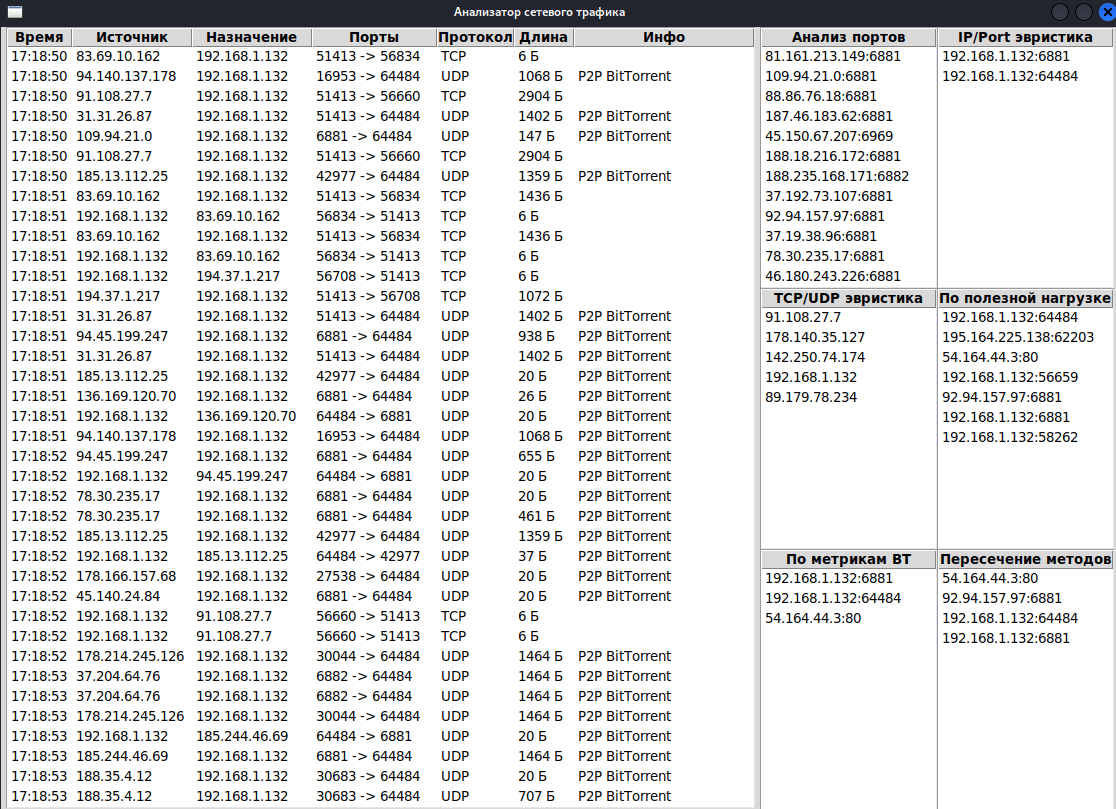
\includegraphics[width=0.999\textwidth]{test3.png}
    \caption{Тестирование программы при запущенном клиенте Bittorrent}
    \label{test3}
\end{figure}

\begin{figure}[H]
    \centering
    \includegraphics[width=0.899\textwidth]{btport.png}
    \caption{Порт входящих соединений qBittorrent}
    \label{btport}
\end{figure}

\newpage
\subsubsection{Запуск программы при запущенном аудио звонке Skype}
На хостовой машине запущен аудио звонок в Skype.

\begin{figure}[H]
    \centering
    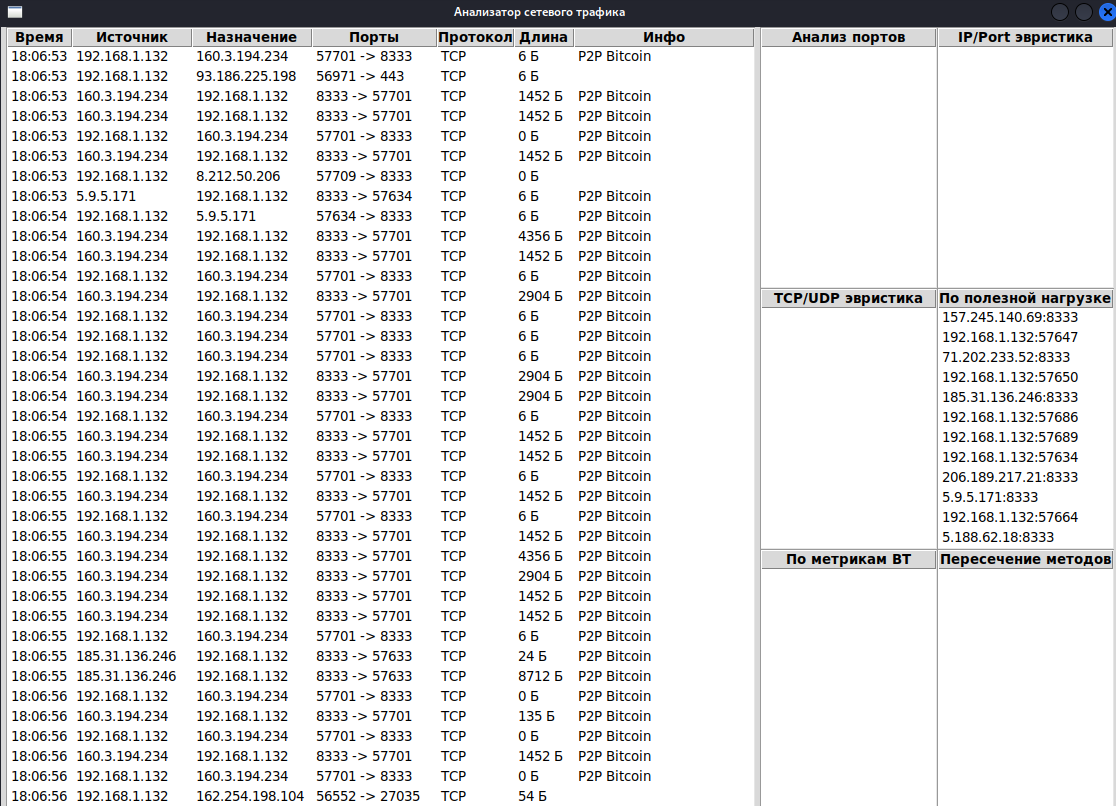
\includegraphics[width=0.999\textwidth]{test4.png}
    \caption{Тестирование программы при запущенном аудио звонке в Skype}
    \label{test4}
\end{figure}

P2P-активность аудио звонка Skype легко обнаруживается с помощью анализа портов (порты 3478 и 3480), поскольку его порты не меняются.

\conclusion
В данной работе были рассмотрены теоретические сведения о технологии P2P: особенности её архитектуры, применение
и способы обнаружения, которые, так или иначе, имеют некоторую степень погрешности. Вместе с тем, были приведены характерные черты такого протокола как Bittorrent, который является одним из самых распространённых среди P2P-сетей.
Поэтому обнаружение Bittorrent можно считать наиболее востребованным.

В практической части была реализована программа "--- сниффер или анализатор сетевого трафика, которая позволяет
перехватывать \textit{TCP} и \textit{UDP} трафик и анализировать его на присутствие P2P-активности. Были реализованы методы анализирования портов и обнаружения TCP/UDP- и IP/Port-эвристики.

Таким образом, изучение P2P-сетей несомненно является актуальным, поскольку они активно используются пользователи Интернета, в следствие чего не останавливается и их развитие. Однако иногда необходимо фильтровать и блокировать P2P-трафик, поэтому необходимо также быстро развивать методы его обнаружения, которые могут устаревать со временем. P2P-протоколы меняют своё поведение, могут использовать случайные номера портов, изменять сигнатуры. Кроме того, многие другие сетевые протоколы могут иметь схожее поведение, поэтому крайне важно различать их между собой, обновлять способы исключения таковых протоколов. Из-за множества подобных факторов не существует универсального способа обнаружения P2P-трафика. Тем не менее, есть необходимое количество узконаправленных методов, которые в совокупности с достаточной 
точностью могут определить P2P-активность в сети.

% \bibliographystyle{gost780uv}
% \inputencoding{cp1251}
% \bibliography{thesis}
% \inputencoding{utf8}

\appendix

    \section{Код \texttt{main.py}}
    \inputminted{python3}{code/sniffer/main.py}

    \section{Код \texttt{sniffer.py}}
    \inputminted{python3}{code/sniffer/sniffer.py}

\end{document}